\blfootnote{Adapted from: Martí-Juan, G., Sanroma-Guell, G., Piella, G. (2020, June 1). A survey on machine and statistical learning for longitudinal analysis of neuroimaging data in Alzheimer’s disease. Computer Methods and Programs in Biomedicine, Vol. 189, p. 105348. \url{https://doi.org/10.1016/j.cmpb.2020.105348}}
\section{Introduction}

Alzheimer's disease (AD) is a neurodegenerative disease that affects millions of elderly people worldwide \cite{Ferri2005,Prince2013}. It is the most common form of dementia worldwide, and it currently has no cure. Cognitively normal (CN) subjects affected with the disease start to show progressive loss of memory and cognition \cite{Backman2004}, entering a mild cognitive impairment (MCI) stage, before developing to full-blown AD. Detecting the disease in its early stages is the key for a more effective treatment aimed at preventing the degenerative process.  \\

An improved understanding of AD progression would be beneficial for early diagnosis of the disease and personalized therapy. AD can be described as a multifactorial disease \cite{Jack2010}. Several biomarkers represent different pathophysiological processes, each with distinct progression paths. Examples of such biomarkers are brain A$\beta$ deposition, tau injury and neurodegeneration, and they can be used to analyze disease progression from different perspectives. \\ 

Due to the widespread use and availability of medical devices during the past decades, we now have access to electronic medical records containing a varied set of clinical data coming from multiple sources, including brain imaging scans from different modalities, acquired over time in a longitudinal fashion \cite{Lawrence2017}.  Contrary to cross-sectional studies, longitudinal studies allow us to measure the evolution and effects of phenotypic characteristics over time caused by disease progression \cite{Mills2014}. \\

Statistical data analysis methods are traditionally used to look for relationships among variables. Machine learning (ML) methods model the relationship between a set of input and output variables and can generalize to unseen data. ML methods can particularly helpful when dealing with high-dimensional data, where traditional statistical methods are not applicable. Such techniques have proven useful for specific tasks (prediction, reconstruction, image segmentation) and to find hidden patterns in the data. Methodologically, the boundary between ML and statistical methods is fuzzy. We refer the reader to \cite{Breiman2001,Shmueli2010} for a more in-depth discussion. \\

Progression of the disease using cross-sectional information has been examined by many ML studies \cite{Oxtoby2017,Acharya2019}. Fewer have used a sequence of acquisitions and assessed longitudinal changes directly. Although working with longitudinal data can improve our knowledge of the disease \cite{Xu2014}, adding a temporal dimension entails difficulties and data analysis problems, such as data imbalance or time alignment, that need to be addressed \cite{Fitzmaurice2008,Ibrahim}. \\

In this survey, we review current machine and statistical learning studies and identify trends for longitudinal medical imaging analysis, current gaps in the literature, and possible future directions. We divide the reviewed studies into two large groups: computer-aided diagnosis (CAD) and progression modelling. We exclude purely statistical inference studies, as our focus is on general-purpose learning techniques. We believe that such techniques can leverage longitudinal information and give new insights into AD and dementia progression, due to their ability to manage and explore growing volumes of diverse available data in an exploratory hypothesis-free setting.\\

%\begin{figure}[ht!]
%  \centering
%  \includegraphics[width=0.95\textwidth]{figures/review/paperoutline.png}
%  \caption{Outline of the review.}
%  \label{fig:overview}
%\end{figure}

% Rewrite this when the figure and the new sections are done
% Figure \ref{fig:overview} shows the outline of the paper. 
This chapter is organized as follows: in Section \ref{sec:search}, we describe the search criteria used to gather the reviewed works. In Section \ref{sec:longdata} we discuss their data usage, focusing on the type of longitudinal data and measured biomarkers. Next, we talk about the tasks addressed by the reviewed works: in Section \ref{sec:progression} we analyze works that model the progression of the disease, categorized by the main method used, and detail the advantages and disadvantages of the reviewed approaches. Then, in Section \ref{sec:classification}, we analyze papers focused on computer-aided diagnosis of the disease, describing both the methods and the data used, as well as their performance. We then discuss specific aspects: in Section \ref{sec:missing}, we explain how researchers handle certain problems such as temporal alignment and missing data approaches. In Section \ref{sec:bias} we discuss the reproducibility and interpretability of the reviewed works. Finally, based on our analysis, in Section \ref{sec:conclusion} we discuss the overall results, draw conclusions, and suggest possible further research paths. \\

\section{Search methods}
\label{sec:search}

We reviewed works that 1) focus on AD or dementia, 2) use medical imaging derived biomarkers, 3) use longitudinal data, and 4) use ML methods. We created four groups of keywords for the search:

\begin{itemize}\itemsep5pt
  \item \textbf{Keywords related to the disease:} Dementia, Alzheimer’s disease, Mild Cognitive Impairment, AD
  \item \textbf{Keywords related to biomarkers of the disease:} MRI, PET, medical imaging, Magnetic resonance imaging, Positron emission tomography, fMRI, T1 MRI, T2 MRI, FLAIR, DWI
  \item \textbf{Keywords related to longitudinal data analysis:} longitudinal, spatiotemporal, temporal, long-term, follow-up, progression
  \item \textbf{Keywords related to machine learning and statistical learning methods:} classification, learning, prediction, data-driven, precision medicine, pattern recognition, artificial intelligence, AI, ML
\end{itemize}

The keywords were chosen to be general terms for each concept but specific enough to discard unrelated papers. We used the search engines of PubMed, ScienceDirect, Scopus, arXiv, and bioRxiv. In each website, we retrieved papers that had at least one keyword from each group. Depending on the website, its search engine did not allow us to use the full search: that was the case in ScienceDirect, Scopus, and Biorxiv, where we had to reduce the number of terms. In these cases, we only used the first two words of each category, which we consider to be the most representative. \\

We excluded papers that were not related to AD or that did not use longitudinal imaging data in their experiments or models. We also excluded papers that did not use a general-purpose learning approach, as mentioned in the introduction. For example, statistical reports whose goal was to test a specific hypothesis. \\

The search was done over a period going from January 1st, 2007 to July 31st, 2019. We obtained a total of 1404 different papers. Then, we removed papers that were out of scope (1300). These include papers that did not use learning methods, that used only cross-sectional data, or that focused on other diseases but had appeared in our search. After that, we removed duplicates from the remaining papers (44), leaving us with a total of 60 papers. Finally, we search on the references and citations of the selected papers to include relevant works that could have been missed by our initial search, adding up to \textbf{105} selected works. Figure \ref{fig:search} shows a diagram of the selection process.

\begin{figure}[!htbp]
  \centering
  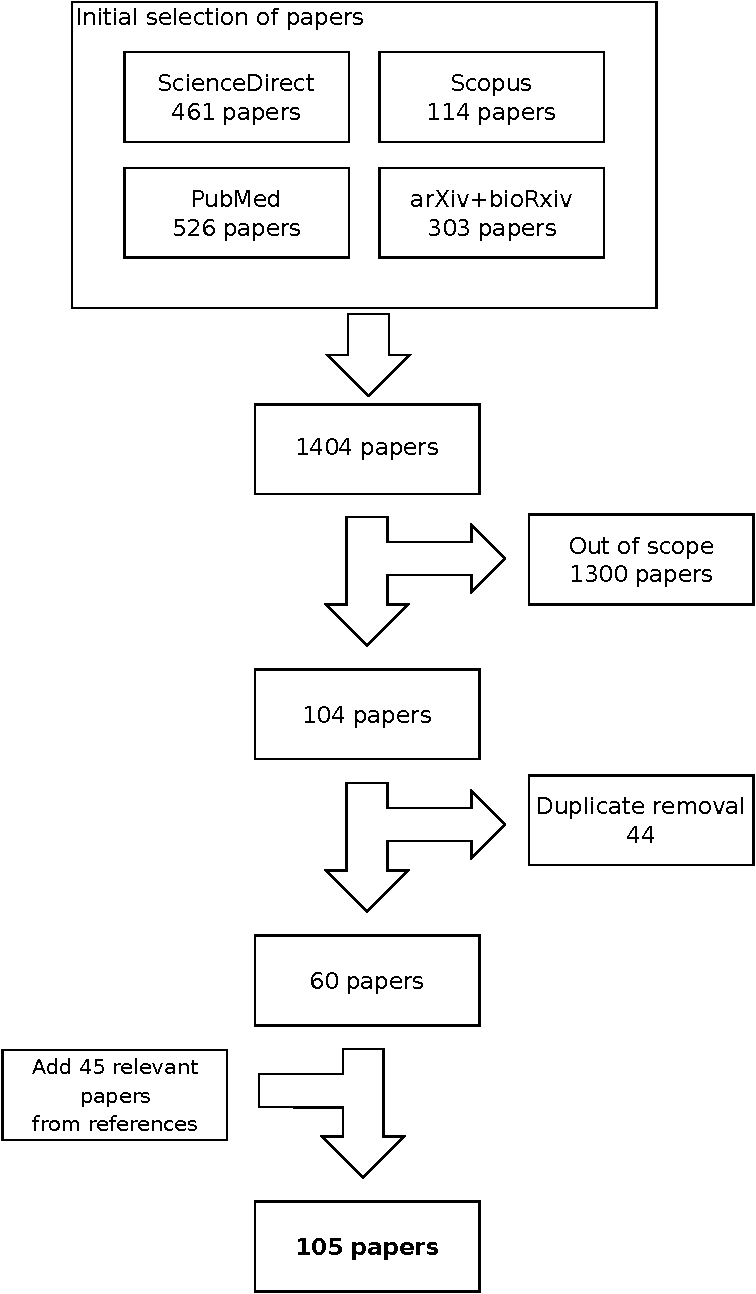
\includegraphics[width=0.9\textwidth,height=0.9\textheight,keepaspectratio]{figures/review/Fig1.pdf}
  \caption{Paper selection pipeline.}
  \label{fig:search}
\end{figure}

\section{Data and methods usage}
\label{sec:longdata}

We analyzed the data and methods in the final selection of papers to gain an initial understanding of the reviewed works. We focused on several key aspects: follow-up length, measured biomarkers, database, and main methods used. \\

\subsection{Follow-up length} 
 
 \begin{figure}[!htbp]
\centering
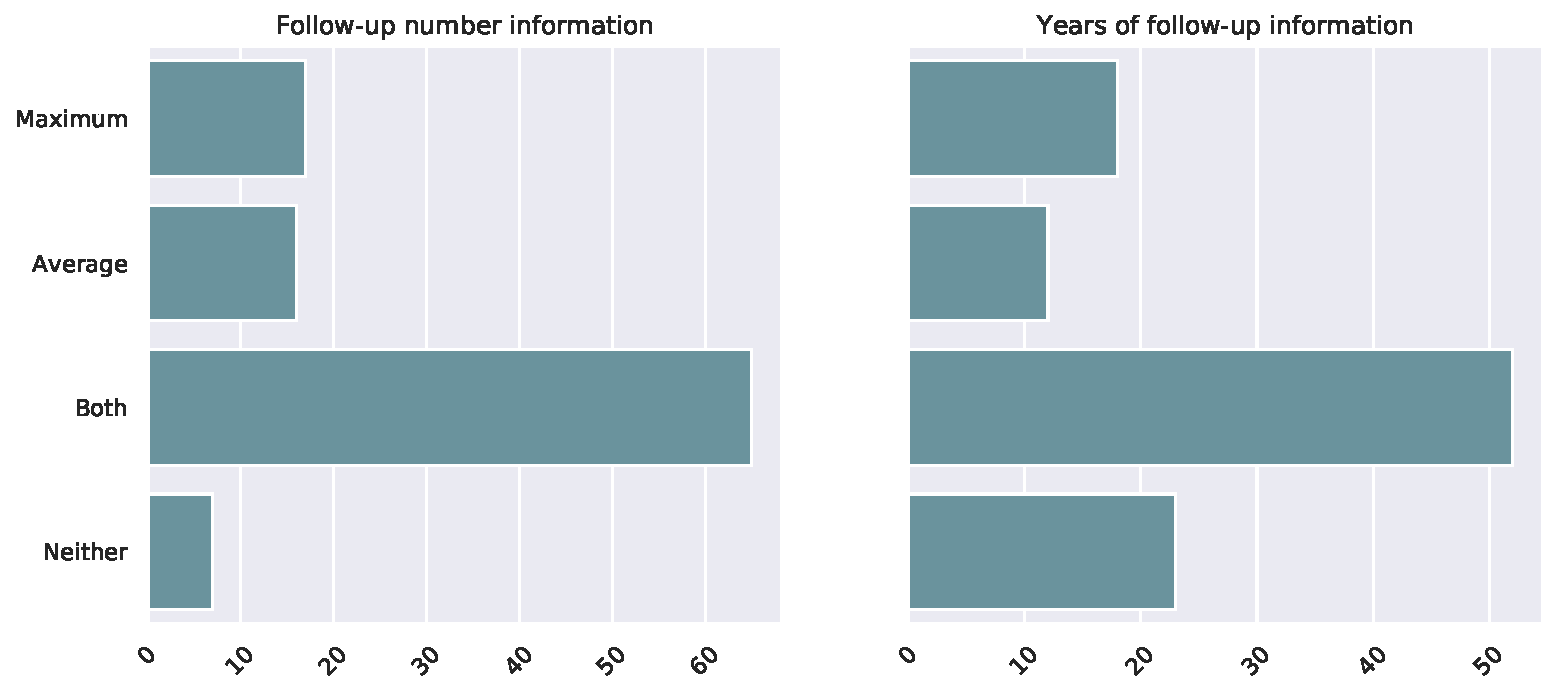
\includegraphics[width=0.95\textwidth]{figures/review/Fig2.pdf}
    \caption{Reviewed papers according to their reporting of follow-up length.}\label{fig:followupsdist}
\end{figure}
 
To assess the impact of longitudinal data used in a paper, we analyzed the number of follow-ups per subject and the follow-up length. Figure \ref{fig:followupsdist} shows how this information was reported in the reviewed articles. Most of them report enough information on the longitudinal data selection, with the majority of articles reporting both the maximum number of follow-ups and the average number of follow-ups, but a sizeable amount of articles did not report information about the years of follow-up. This can raise some concerns about reproducibility (see Section \ref{sec:bias}), and it affects the comparison with other works and the correct assessment of the methodology used. \\

Figure \ref{fig:followups} shows the distribution of the (maximum and/or average) number of follow-ups reported in the selected papers. We observe that the distribution is skewed at a low number of follow-ups, in both maximum- and average-number graphs. This is an expected result due to the limited availability of adequate long-term data: subjects having a large number of follow-ups are sparse in available longitudinal datasets \cite{Lawrence2017}. A substantial percentage of works ($39\%$, not counting those that did not report the information) use only one or two follow-ups in addition to the baseline. \\

\begin{figure}[!htbp]
\centering
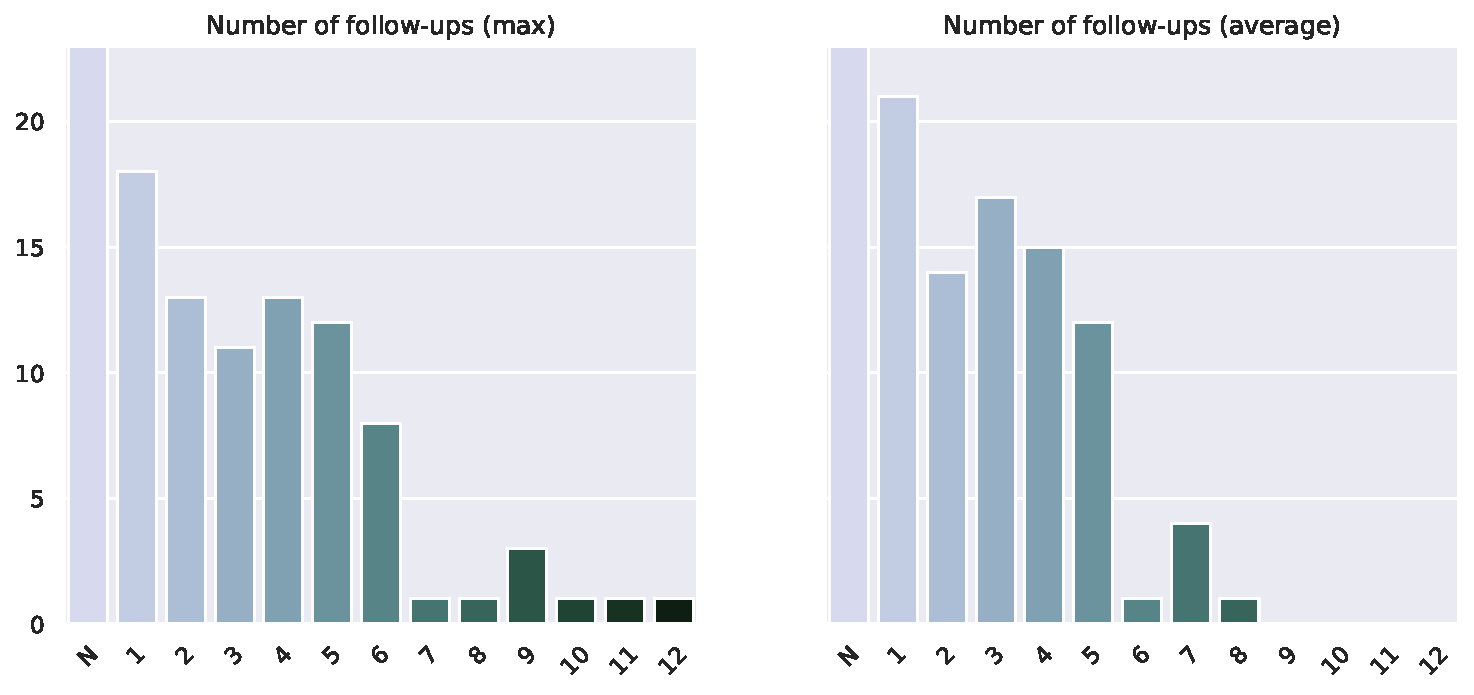
\includegraphics[width=1.0\textwidth]{figures/review/Fig3.pdf}
    \caption[Distribution of the number of follow-ups used in the reviewed papers.]{Distribution of the number of follow-ups (maximum and average) used in the reviewed papers. Rounded average values. N: not reported.}\label{fig:followups}
\end{figure}

Figure \ref{fig:followups_years} shows the distribution of the (maximum and/or average) number of years of follow-up reported. In average, studies follow the patients for between 1 to 3 years, and a maximum of 2 to 4 years. There is a small subset of papers that are very long term following the patient from 8 to 12 years \cite{Ghazi2019,Chen2012,Li2017b,Li2017c,Bilgel2015a,Bilgel2016}. Depending on the follow-up length, we distinguish between two groups:

\begin{figure}[!htbp]
\centering
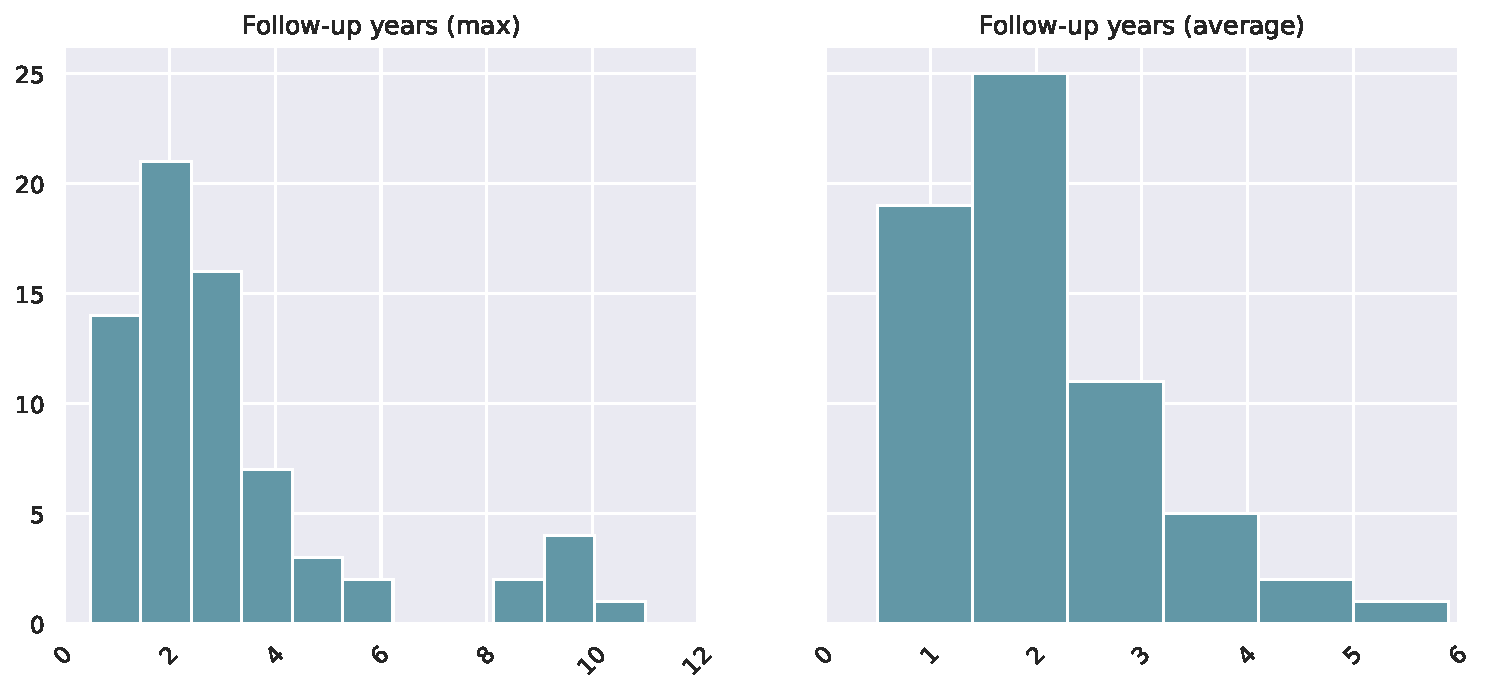
\includegraphics[width=1.0\textwidth]{figures/review/Fig4.pdf}
    \caption[Distribution of the years of follow-up used in the reviewed papers.]{Distribution of the years of follow-up (maximum and average) used in the reviewed papers.}\label{fig:followups_years}
\end{figure}

\begin{itemize}\itemsep7pt

\item Short-term longitudinal works, including follow-ups up to, at maximum, two years. These papers tend to select a subset of available data, avoiding missing data and unbalanced data problems \cite{Ardekani2016,Fiot2012,Fiot2014,Gray2012,Rodrigues2014,Shi2015,Shi2017}. Papers based on short-term brain atrophy \cite{Huang2012,Hyun2016,McEvoy2011,Sanroma2017,Vounou2012}, where usually only one follow-up is needed to calculate tissue loss, and those using several modalities that want to avoid missing data problems \cite{Chen2011b,Hinrichs2011,Jack2009} tend to be short-term.

\item Long-term longitudinal works, including follow-ups of three years or more. These papers need to deal with missing data, as long-term data tend to be sparse. However, long-term data give additional insight into the whole progression of the disease that short-term longitudinal data cannot provide. There are many disease progression studies using long-term longitudinal data \cite{Desikan2011,Guillaume2014,Guerrero2016,Bilgel2015a,Bilgel2016,Iturria-Medina2016,Li2017b,Aghili2018}, whereas computer-aided diagnosis works using long-term longitudinal data are less common \cite{Chi2017,Minhas2016}. Some works use longer-term longitudinal data for model validation after training on a short-term subset \cite{Young2015a}.
\end{itemize}

As mentioned before, subjects with a large number of follow-ups are limited \cite{Lawrence2017}. This is due to various reasons: dropout from the study, missing data due to faulty screenings, and short follow-up time, among others. Even if the number and length of follow-up measures may increase over time, dropout of patients and missing data are phenomena that are present in longitudinal studies. In Section \ref{sec:missing} we give examples of the methods used by researchers to overcome those problems. \\

\subsection{Data sources}

Longitudinal data used in the reviewed papers come from diverse studies. An in-depth review of available longitudinal studies that measure AD biomarkers can be found in \cite{Lawrence2017}. Figure \ref{fig:db} shows the distribution of databases used in the reviewed papers.  \\

\begin{figure}[!htbp]
  \centering
  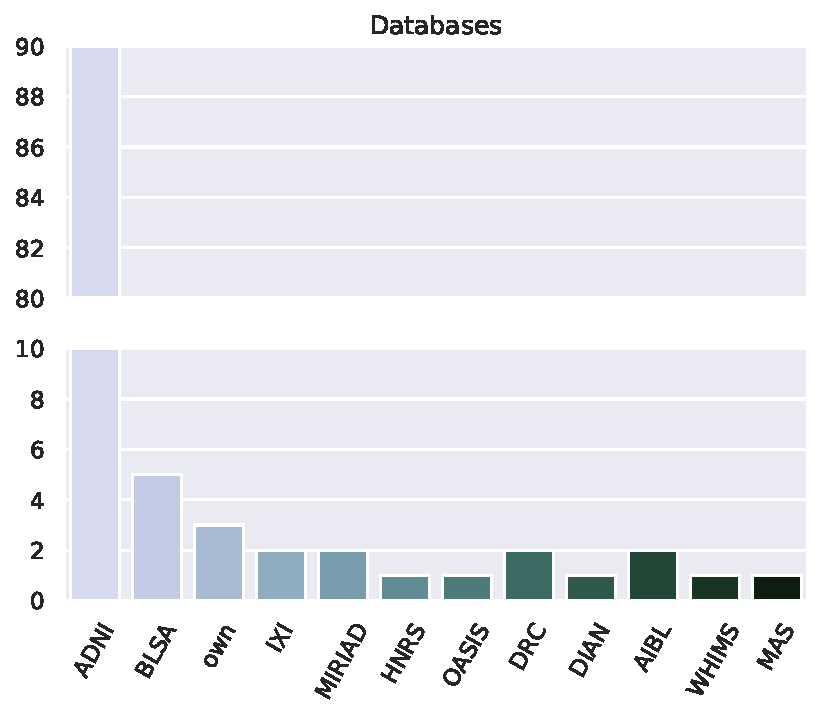
\includegraphics[width=0.75\textwidth]{figures/review/Fig5.pdf}
  \caption[Distribution of longitudinal studies used in the reviewed papers.]{\small Distribution of longitudinal studies used in the reviewed papers. The graphic is truncated to represent higher counts. ADNI: Alzheimer's Disease Neuroimaging Initiative, BLSA: Baltimore Longitudinal Study of Aging, own: own datasets, not public and/or gathered inhouse, IXI: Information eXtraction from Images, MIRIAD: Minimal Interval Resonance Imaging in Alzheimer's Disease, HNRS: Heinz Nixdorf Recall Study, OASIS: Open Access Series of Imaging Studies, DRC: Dementia Research Centre, DIAN: Dominantly Inherited Alzheimer Network, AIBL: Australian Imaging, Biomarker $\&$ Lifestyle Study of Ageing, WHIMS: Women's Health Initiative Memory Study, MAS: Sydney Memory and Aging Study}\label{fig:db}
\end{figure}

ADNI \cite{Weiner2017} is the most used database, being the largest public longitudinal database for AD patients in the world. It has well organized and processed data, and it has many different modalities and long follow-up times. Also, obtaining access to ADNI data is easy and fast. With all these characteristics, it is not surprising that ADNI is the most widely published dataset. Other databases are less popular due to their lower amount of data, limited/smaller number of modalities, or difficulty to access them, and often they are used together with ADNI \cite{Davatzikos2009,Eshaghi2017,Franke2012} as a separate testing set. Some datasets are more specific regarding, for example, the type of patients they have (Sidney MAS, DIAN, WHIMS) or their follow-up criteria. Interestingly, the Rotterdam elderly study \cite{Ikram2017} was not used in our reviewed studies, given its size and popularity. However, given that it is not specifically focused on AD and that it has more complicated access permission, it is reasonable to think that no studies done with this dataset fit our criteria.  \\

Having a predominant database allows for more direct comparisons between results obtained by different methods. However, this can also lead to a generalization problem, where methods would be specific to ADNI's dataset domain but would not extrapolate to the general population. Using an independent (out-of-study) dataset to test the method is advisable to detect this problem, but those are not always available. Data accessibility in medical imaging is a complicated issue due to privacy concerns, which complicates the availability of public datasets. \\

\subsection{Biomarkers}

Many works use biomarkers from different sources to characterize different AD processes. Figure \ref{fig:modalities} shows the distribution of biomarkers used in the selected papers. We observe that magnetic resonance imaging (MRI) is, by far the most used type of data. Other modalities, such as positron emission tomography (PET) images with different contrasts or cerebrospinal fluid (CSF) biomarkers, receive low attention despite their importance for disease stratification and early detection \cite{Andreasen1999,Clark2011,Weiner2005}, and are often used in combination with other modalities. Due to their more invasive acquisition methods, they are not as widely available as MRI in longitudinal studies and are more prone to missing acquisitions. \\

\begin{figure}[!htbp]
\centering
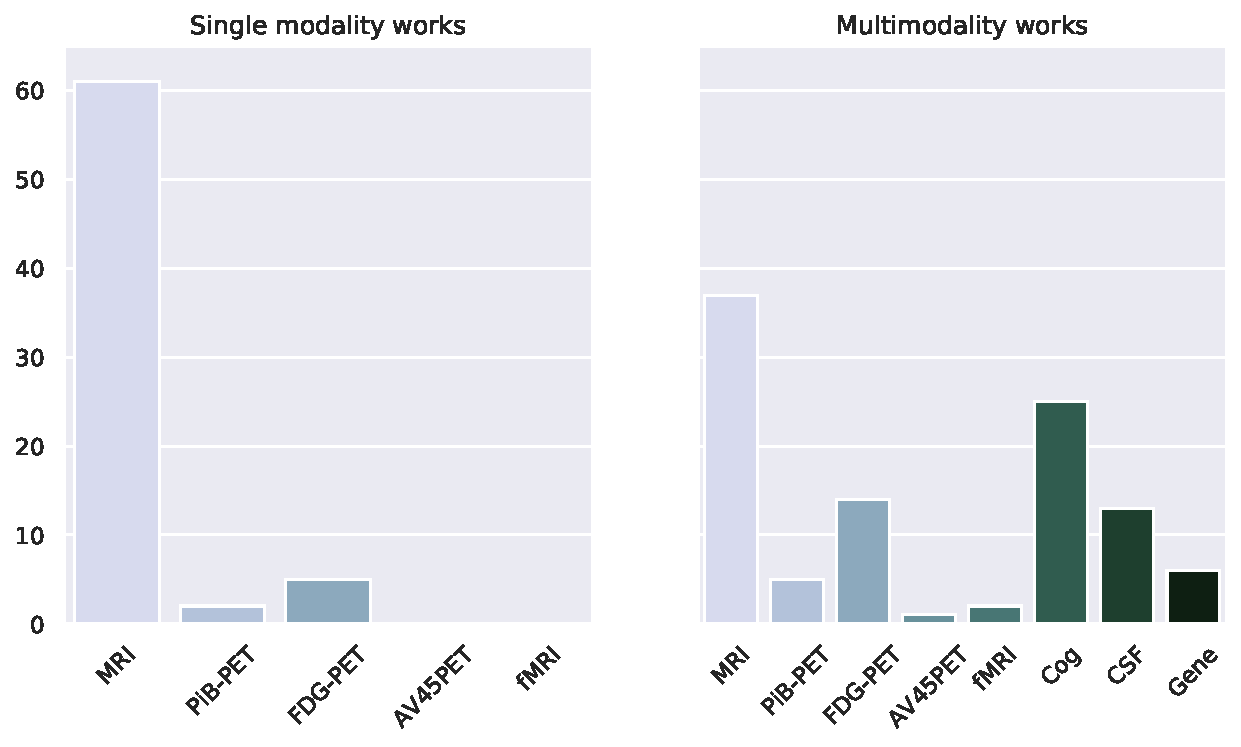
\includegraphics[width=0.73\textwidth]{figures/review/Fig6.pdf}
    \caption[Distribution of measured biomarkers, for single- and multimodality papers.]{\small Distribution of measured biomarkers, for single- and multimodality-based papers. MRI:  magnetic resonance imaging. PET: positron emission tomography, PiB: Pittsburgh compound B, FDG: fluorodeoxyglucose, AV45: Florbetapir AV-45, fMRI: functional MRI, Cog: cognitive assessments, CSF: cerebrospinal fluid, Gene: genetic biomarkers, Plasma: plasma biomarkers, DTI: diffusion tensor imaging.}\label{fig:modalities}
\end{figure}

\subsection{Methods}

Table \ref{table:methods} shows the main methods used by the articles reviewed in this paper. Those methods can be categorized into two groups according to the task they aim: progression models, which seek to quantify the evolution of the disease; and classification models, which predict diagnosis labels of patients. Some of the methods, such as deep learning or multi-task learning, are flexible and can be used for both tasks. Moreover, some works use several different methods for their objectives. The list in \ref{table:methods} is not exhaustive, but it provides a general picture of the current approaches in the field. For classification, support vector machines (SVM) are the most popular model, whereas for progression, a wider variety of methods are employed. In the next sections (Section \ref{sec:progression} and \ref{sec:classification}) we discuss and compare the aforementioned methods. 

\begin{table}[htbp]
\centering
\resizebox{0.75\textwidth}{!}{%
\begin{tabular}{@{}cC{5cm}@{}}
\toprule
Method                        & References \\ \midrule
Multi-task learning           & \cite{Liu2013,Thung2016,Zhang2017,Zhou2013a,Thung2018,Yang2018,Aksman2019}    \\   
Deep Learning                 & \cite{Ghazi2019,Givon2017,Ortiz2017,Cui2018,Aghili2018,Bhagwat2018}    \\
Event-based models            & \cite{Fonteijn2012,Oxtoby2018}    \\
Manifold learning             & \cite{guerrero,Wolz2010,Guerrero2015}    \\
Mixed effect models           & \cite{Bilgel2016,Dodge2014,Guerrero2016,Iturria-Medina2016,Koval2018,Li2017c,miriad,Schiratti2015,Ziegler2015b}    \\
Shape analysis models         & \cite{Gui2017,Tang2015,Bone2017,Bone2018,Gutman2013,Eshaghi2017}    \\
Gaussian processes            & \cite{Hyun2016,Lorenzi2015b,Lorenzi2015c,Lorenzi2017}    \\
Data-based progression scores & \cite{Bilgel2015a,Franke2012,Gaser2013,Jedynak2012,Casanova2018}    \\
Support Vector Machine        & \cite{Aksman2016,Cabral2015,Chen2011b,chincarini,Clark2012,Davatzikos2009,Farzan2015,Gavidia-Bovadilla2017,Gray2012,Lei2017,Li2012,Misra2009,Rodrigues2014,Shi2017,Sun2017,Zhang2017a,Zhu2016a,Adaszewski2013,Guan2017}    \\
Multiple Kernel learning      & \cite{Chen2015,Hinrichs2011,Zhang2012a}    \\
Logistic Regression           & \cite{Fiot2012,Fiot2014,Sanroma2017,Vounou2012}    \\
Random Forests                & \cite{Ardekani2016,Huang2016c,Mubeen2017}    \\ \bottomrule
\end{tabular}}
\caption{Main methods used in the reviewed papers.}\label{table:methods}
\end{table}

\section{Progression models}
\label{sec:progression}

Models of disease progression can be used to quantify the evolution, determine temporal trajectories, and detect different paths of degeneration, among other sub-tasks. In this section, we comment on approaches that build disease progression models from longitudinal data, grouping them by their general methodology. \\

\subsection{Multi-task learning for cognitive prediction}

Predicting the rate of cognitive decline from imaging biomarkers can be useful to detect brain regions that directly affect cognitive evolution. Besides, cognitive performance can provide a continuous measure related to disease progression that may complement the categorical information about diagnosis. Since several cognitive scores of the patient are often available, multi-task learning is a popular approach for cognitive prediction. Defining cognitive scores as separate prediction tasks and training them jointly creates a more robust predictive model. Such models have shown to have many advantages: they can use a variable number of follow-ups \cite{Lei2017,Zhou2013a,Aksman2019} and can provide direct information between cognitive scores and imaging biomarkers \cite{Jie2017,Lei2017,Wang2012b,Wang2016,Zhang2012a}. Apart from multi-task learning, other methods have been used for this task, such as probabilistic models \cite{Zhu2018}, regression models \cite{AraqueCaballero2017}, or learning ensemble models \cite{Chi2017,Huang2016c,Yang2018a}, which combine different, smaller models, and can be defined in flexible ways to integrate missing follow-ups into the model. \\

\subsection{Deep learning}

Deep learning (DL) is a powerful representation technique that is state of the art in many ML problems. A DL model is a neural network with many layers, which can learn from large amounts of data to do specific tasks. For a comprehensive review of DL techniques in medical imaging, we refer the reader to Litjens et al.\ \cite{Litjens2017}. \\

Convolutional neural networks (CNN), which are commonly applied to images, have been used for cognitive score prediction \cite{Givon2017,Zhang2017}. In Zhang et al.\ \cite{Zhang2017}, they combined CNN and MTL, using CNN-based features to train an MTL-based model. In a different approach, Givon et al.\ \cite{Givon2017} proposed a CNN architecture that can predict the cognitive score of the patient at any time, not being restricted to existing follow-ups. \\

Recurrent neural networks (RNN) are networks where previous outputs are used as inputs while having hidden states. Due to this, they are said to have memory and can model sequential data. Consequently, RNN have the potential to be able to learn from longitudinal data. They have already been used to predict the progression of AD using diverse cognitive scores \cite{Wang2018}, but without imaging information. \cite{Ghazi2019,Cui2018,Aghili2018} all used RNN with imaging biomarkers, although not to quantify progression but for computer-aided diagnosis. Despite their popularity in other fields, RNN are still not widely used for modelling disease progression using medical imaging. A possible reason could be that DL methods are mostly non-interpretable, and any performance gains do not usually compensate for the loss in interpretability. \\ 

\subsection{Event based models}

Event-based models (EBM) \cite{Fonteijn2012} are a modelling approach that describe a neurodegenerative disease by an ordered series of events, such as the appearance of a new symptom. EBM define a fixed number of biomarkers, modelling each of them separately to obtain a distribution of abnormal and normal values (indicating the presence of the disease or not) and to generate an ordering of events. We can use this ordered sequence of events to assess the disease stage. \\

In their initial formulation, EBM were not well-suited to accommodate longitudinal data. There are several studies based on EBM for modelling disease progression that use longitudinal data, either by using biomarkers derived from brain atrophy rates \cite{Fonteijn2012,Huang2012,Young2014} or because they validated their results using the available longitudinal information \cite{Oxtoby2018,Young2014}. Given the potential and strong results they show, integrating longitudinal data in such models is a promising research direction. \\

\subsection{Manifold learning}

Manifold learning is an approach to dimensionality reduction. It assumes that the high-dimensional data lie (at least approximately) on a manifold of much lower dimension. Applied to disease progression modelling, manifold learning can be used to estimate an underlying subspace where longitudinal patient trajectories can be better represented. These are directly learnt from the data, and typical problems such as temporal alignment and unbalanced datasets are solved in the subspace learning process. Wolz et al.\ \cite{Wolz2010} used Laplacian eigenmaps to build a longitudinal manifold, where AD and CN subjects are well differentiated. Guerrero et al.\ \cite{Guerrero2015,guerrero} also proposed a method based on Laplacian eigenmaps, adding a constraint to limit connections between scans from the same subject, to create a temporal embedding that shows the progression of the patient. \\

These methods are not as popular as other types of progression models: they are not as directly interpretable as other models such as EBM or multi-task learning and can be much more complex to implement. However, one can introduce interpretability by effectively embedding the progression in a relevant low-dimensional manifold. This, together with their potential to integrate contextual information (e.g. constraints on longitudinal data \cite{Guerrero2015}), makes manifold learning an underrated approach for disease progression.

\subsection{Mixed effect models}

Mixed effect models are widely used due to their flexibility to deal with unbalanced data, and their ability to naturally model average disease progression (fixed effects) and inter-subject variability (random effects). They are commonly considered a classical statistical technique, but we decided to include works that used such models to observe and quantify progression, due to their importance in longitudinal analysis. Bernal-Rusiel et al.\ \cite{Bernal-Rusiel2013} presented an overview of these methods for MRI, suggesting that linear mixed effect models detect MRI longitudinal group differences with more sensitivity and specificity than other methods such as ANOVA or general linear models, especially with unbalanced datasets. \\

Mixed effect models have been extensively used in longitudinal progression models for AD \cite{Bilgel2015a,Bilgel2016,Davatzikos2009,Koval2018,miriad,Platero2019,Schiratti2015,Villemagne2013,Ziegler2015b}, as they can be directly adapted to unbalanced longitudinal datasets \cite{Koval2018}, extended by adding priors such as genetic biomarkers \cite{Ziegler2015b} or different progression speeds and disease onset \cite{Schiratti2015}, or used to derive new data-based biomarkers that reflect the progression of the disease \cite{Bilgel2015a,Bilgel2016,Davatzikos2009,Platero2019}. Apart from MRI, linear mixed models have also been applied to other biomarkers, such as PET-based biomarkers \cite{Bilgel2016,Dodge2014}. \\

Mixed effect models are easily adapted to more than one modality of data. For this reason, they have also been used extensively in longitudinal multimodal analysis. The easiest way to use them with multiple modalities is to define a different model for each modality \cite{Dodge2014,Guerrero2016,Li2017c}, allowing us to draw comparisons between biomarkers \cite{Jedynak2012} or to combine them to show the overall progression of the patient \cite{Bilgel2015a,Bilgel2016,Donohue14,Jedynak2012,Li2017a}. This combination usually needs a type of temporal alignment of the biomarkers (see Section \ref{subsec:tempalig}) prior to fitting the model \cite{Guerrero2016}, by using a defined scale such as cognitive scores \cite{Yang2011}, or directly in the fitting model \cite{Li2017a}. Iturria-Medina et al.\ \cite{Iturria-Medina2016} applied a multifactorial mixed model to one of the largest patient cohorts in the field, with more than 7700 images and biomarkers from 1100 patients at various stages of the disease, to model and explore the evolution of different biomarkers. Their results suggest that vascular dysregulation might be the earliest factor associated with AD development. 

\subsection{Shape analysis models}

Some methods focus on modelling shape changes in certain brain regions during the disease. This allows capturing subtle variations between or within subjects, which would be lost just by looking at flat imaging biomarkers such as volume or voxel intensity. Current research shows longitudinal changes in shape in key structures of the brain (such as lateral ventricles or hippocampus) that are strongly related to cognitive degeneration \cite{Gui2017,Tang2015} and can reveal differences between groups of patients \cite{Bone2017,Bone2018,Gutman2013}. Mixed effect models are often used for modelling shape changes \cite{Bone2017,Bone2018,Gui2017,Tang2015}, with Eshaghi et al.\ \cite{Eshaghi2017} proposing a novel vertex clustering method to model shape changes over time, using a similar mixed effect model already proposed in other reviewed works \cite{Donohue14,Jedynak2012,Schiratti2015}.

\subsection{Other models}

Besides the methods discussed so far, other types of models for disease progression are also used.  Generalized estimation equations for longitudinal analysis \cite{liang1986longitudinal} model both the mean response of a population and the covariance of repeated measures \cite{Zhang2014}, and deal with unbalanced datasets \cite{Guillaume2014,Li2013}. Gaussian processes are also used to model spatio-temporal changes and dependencies \cite{Hyun2016,Lorenzi2015b,Lorenzi2015c} and to integrate different modalities \cite{Lorenzi2017}. Some methods focus on specific tasks, such as finding hidden latent temporal factors of the disease \cite{Chen2012,Wachinger2017}, or are specifically designed to tackle problems such as unbalanced data or patient alignment \cite{Bilgel2018,Dawson2016,Goyal2018,Li2013}. In Liu et al.\ \cite{Liu2015} they used a non-linear atlas-based model to simulate future MRI scans from previous follow-ups, similar to \cite{Lorenzi2015c}. Other papers focus on specific data or biomarkers, such as brain connectivity \cite{Chenhui2014} or functional data \cite{Li2017b}.  \\

\cite{Franke2010,Franke2012,Gaser2013} defined a method that aggregates the ageing change over time into a single biomarker and compared it to the real age of the patient and its evolution across time. Atrophy of the brain due to dementia can be similar to atrophy due to normal ageing: brain atrophy can occur because of both normal ageing and pathological reasons. Disentangling those two sources can be useful to discover the disease earlier. In the same line, Lorenzi et al.\ \cite{Lorenzi2014} proposed a non-rigid registration method to disentangle the contributions of normal atrophy and disease atrophy, and observed their relation to AD progression. This age-based approach allows us to introduce prior knowledge about healthy subjects in the model and then study the deviations that appear. Such an idea has been used in computer-aided diagnosis with remarkable results \cite{Gavidia-Bovadilla2017}. \\

For multimodal data, we find works combining genetic information with imaging biomarkers, using regression-based models \cite{Silver2012,Vounou2012}, which are useful to discover longitudinal interactions between imaging biomarkers and genetic factors that could go unseen in cross-sectional analysis \cite{Xu2014}. Creating data-based progression scores \cite{Casanova2018,Clark2012,Davatzikos2009,Jedynak2012,Schmidt-Richberg2015} is also a recurrent approach to quantify progression, independently of the method chosen, because such scores are easy to interpret and compare against. Goyal et al.\ \cite{Goyal2018b} applied hidden Markov models, using different biomarkers, to characterize the progression of the disease into stages, and discovered two different paths of AD progression. Recently, Marinescu et al.\ \cite{Marinescu2019} proposed a vertex-wise progression model over the cortical surface which can be used in different diseases and with different biomarkers to recover and estimate patterns of brain pathology. They test the model on real and simulated data and it is shown to have potential clinical relevancy. Using multimodal data can also be useful to find subtypes of the disease, given its heterogeneity \cite{Gamberger2017}. Thus, combining longitudinal multimodal data is effective to discover hidden AD factors unseen in cross-sectional or single-modal data. \\

\section{Computer-aided diagnosis}
\label{sec:classification}

Many ML approaches to AD focus on computer-aided diagnosis (CAD): given data about patients, the objective is to classify them depending on their diagnosis (CN, MCI, or AD). An extension of this task is to distinguish between MCI patients that will convert to AD (MCIc), and those that will not convert and remain stable (MCInc), which is useful for early detection of the disease. Cross-sectional imaging data have been used extensively for this task, and we refer the reader to Rathore et al.\ \cite{Rathore2017} for an in-depth review. In this section, we study works dealing with this problem using novel methods to process and interpret longitudinal data. We present first papers using exclusively structural MRI (which are the majority), and then those using other modalities. Finally, we comment on the general performance of the methods. \\

\subsection{Computer-aided diagnosis - structural MRI}

A large percentage of the reviewed works use structural MRI as their main source of data, and CAD focused works are no exception, given that structural MRI is considered a clinical predictor of AD \cite{Adaszewski2013}. Table \ref{table:cadmri} shows the performance and principal characteristics of the reviewed works using (exclusively) MRI on CAD. We have divided them by their use of MRI data to build their model: voxel-wise methods and region of interest (ROI) based methods. Some of the works focus only on the hippocampus. \\ 

% VOXEL BASED METHODS
Whole brain voxel-wise analysis allows detecting relations across the whole brain, not being restricted to parcellations. However, this results in high-dimensional input data, which often requires feature selection and/or dimensionality reduction. One way to do it is to detect landmarks across the brain and extract features around those marks \cite{Farzan2015,Zhang2017a}. Other methods are principal component analysis (PCA) \cite{Aksman2016,Farzan2015,Sun2017}, regularization \cite{Ortiz2017} or metric learning \cite{Shi2015}. All these methods need to capture the differences/changes in voxels across time and use them as features. This can be done by computing some difference between the images, such as brain volume changes \cite{Farzan2015}, or deformation maps across follow-ups \cite{Davatzikos2009,Misra2009,Sun2017}. In Huang et al.\ \cite{Huang2016b}, they used a hierarchical regression classifier on longitudinal voxel selection features that solves both problems: selecting the voxels using an individual classifier for every single voxel in the brain, and training the classifiers with the longitudinal data. In a more recent study, Cui et al.\ \cite{Cui2018} used two different neural networks (multi-layer perceptrons and gated recurrent units) to extract spatial and longitudinal features from MRI images. \\ 

% Other regions
ROI-based methods use a parcellation of the brain to extract features, limiting their amount and avoiding the curse of dimensionality. Studies use a variety of popular methods, such as support vector machines (SVM) \cite{Gavidia-Bovadilla2017,Guan2017,Li2012,Zhu2016a}, multi-task learning \cite{Liu2013}, or RNN \cite{Ghazi2019}, extending them to account for longitudinal data. For example, Zhu et al.\ \cite{Zhu2016a} defined a stratified SVM method to enforce temporal consistency across follow-ups, and Gavidia-Bovadilla et al.\ \cite{Gavidia-Bovadilla2017} created null models of normal ageing using non-demented subjects, and training an SVM with the residuals. Those two methods illustrate how prior knowledge of the dynamics of the disease (non-reversible nature of AD and deviation from normal ageing, respectively) can be incorporated into a ML model. \\

% REGION BASED METHODS
The hippocampus is one of the earliest affected brain regions in AD \cite{Ballard2011}. Consequently, many works have focused on this region \cite{chincarini,Shi2017}, specially for MCIc vs MCInc classification \cite{Fiot2014,Sanroma2017}. We observe a variety of methods to extract meaningful features from the hippocampus: patch-based atrophy descriptors \cite{Sanroma2017}, longitudinal segmentation methods \cite{Platero2019}, non-linear metric learning and autoencoders \cite{Shi2017}, longitudinal deformation \cite{Fiot2012,Fiot2014} and hippocampus volume change \cite{chincarini}. These last two articles also compare different processing methods and their performance to further validate their approach. \\ 

% conclusions
Among the reviewed papers, SVM is the most used classification method (see Table \ref{table:cadmri} due to its simplicity, availability, and strong performance. However, DL methods are gaining popularity, using CNN \cite{Ortiz2017} and RNN \cite{Ghazi2019,Cui2018}. \\

\begin{sidewaystable} % <-- HERE
\centering
\resizebox{0.95\textwidth}{!}{%
\begin{tabular}{@{}lcccccllllccc@{}}
\toprule
Study & \multicolumn{4}{c}{Subjects} & Scans & Type & Algorithm & Database & Validation & \multicolumn{3}{c}{Classification results} \\ \cmidrule{2-5} \cmidrule{11-13}
 & CN & sMCI & pMCI & AD & & & & &  & AD/CN & MCI/CN & sMCI/pMCI \\ \midrule
Misra et al.\ \cite{Misra2009} & - & 76 & 27 & - & 3 & V & SVM & ADNI & LOOCV & - & - & 81.5 \\
Adaszewski et al.\ \cite{Adaszewski2013} & 83 & 61 & 142 & 83 & 7 & V & SVM & ADNI & BS & - & - & 62 \\
Farzan et al.\ \cite{Farzan2015} & 30 & - & - & 30 & 3 & V & SVM &  ADNI & LOOCV & 91.7 & - & - \\ 
Shi et al.\ \cite{Shi2015}  & 123 & 121 & - & 94 & 2 & V & SVM & ADNI & CV & 88.4 & 86.5 & - \\
Huang et al.\ \cite{Huang2016b} & - & 61 & 70 & - & 7 & V & LSR & ADNI & CV & - & - & 79.4 \\
Aksman et al.\ \cite{Aksman2016} & 148 & 148 & - & - & 2 & V & SVM & HNRS,OASIS & CV & - & 74.3 & - \\
Ortiz et al.\ \cite{Ortiz2017}  & 68 & - & - & 70 & 6 & V & DL & ADNI & CV & 94 & - & - \\
Cui et al.\ \cite{Cui2018} & 229 & - & - & 198 & 5 & V & RNN & ADNI & CV & 89.69 & - & - \\  \midrule
Sun et al.\ \cite{Sun2017} & - & 47 & 63 & - & 5 & V & SVM & ADNI & CV & - & - & 92 \\
Zhang et al.\ \cite{Zhang2017a}  & 207 & 346 & - & 154 & 6 & V & SVM & ADNI & CV & 88.3 & 79.02 & - \\ 
Li et al.\ \cite{Li2012} & 40 & 36 & 39 & 37 & 5 & ROI & SVM & ADNI & LOOCV & 96.1 & - & 81.7 \\
Liu et al.\ \cite{Liu2013} & - & 185 & 164 & - & 5 & ROI & MTL & ADNI & LOOCV & - & - & 71.4 \\
Thung et al.\ \cite{Thung2016} & - & 53 & 60 & - & 4 & ROI & MKL & ADNI & CV & - & - & 78.2 \\
Zhu et al.\ \cite{Zhu2016a} & - & 81 & 70 & - & 5 & ROI & SVM & ADNI & CV & - & - & 76.5 \\ 
Gavidia-Bovadilla et al.\ \cite{Gavidia-Bovadilla2017} & 215 & 366 & - & 166 & 8 & ROI & SVM & ADNI & CV & 94.1 & 83.8 & 76.7 \\ 
Ghazi et al.\ \cite{Ghazi2019} & \multicolumn{4}{c}{742} & 12 & ROI & DL+LDA & ADNI & - & 0.9$^{b}$  & 0.59$^{b}$  & 0.78$^{b}$  \\ \midrule 
Fiot et al.\ \cite{Fiot2012} & - & 84 & 19 & - & 2 & H & LGR & ADNI & CV & - & - & 0.65/0.62$^{c}$ \\
Fiot et al.\ \cite{Fiot2014} & - & 84 & 19 & - & 2 & H & LGR & ADNI & CV & - & - & 0.46/0.84$^{c}$ \\
Chincarini et al.\ \cite{chincarini} & 148 & 95 & 121 & 96 & 3 & H & SVM & ADNI & CV & - & 0.88$^{b}$  & - \\ 
Sanroma et al.\ \cite{Sanroma2017}  & - & 100 & 164 & - & 2 & H & LGR & ADNI & CV & - & - & 76.6 \\
Shi et al.\ \cite{Shi2017} & 123 & 121$^{a}$ & - & 94 & 2 & H & SVM & ADNI & CV & 85.9 & - & 76.7 \\
Platero et al.\ \cite{Platero2019} & 137 & 82 & 101 & 77 & 4 & H & LDA & ADNI,MIRIAD & BS & 0.947$^{b}$ & 0.805$^{b}$ & - \\
 \bottomrule
\end{tabular}}
\caption[Performance of reviewed computer-aided diagnosis papers using longitudinal structural MRI.]{\footnotesize Performance of reviewed computer-aided diagnosis papers using longitudinal structural MRI. SVM: Support vector machine, LSR: Least squares regression, LGR: Logistic regression, MTL: Multi task learning, MKL: Multiple kernel learning, DL: Deep learning, LDA: Linear discriminant analysis, V: Voxel-wise, ROI: Region of interest, H: Hippocampus, ADNI: Alzheimer’s Disease Neuroimaging Initiative, HNRS: Heinz Nixdorf Recall Study, OASIS: Open Access Series of Imaging Studies. CV: k-fold cross-validation. LOOCV: Leave one out cross-validation. BS: Bootstrapping. If the number of scans is variable, the maximum is reported. \\
         $^{a}$ MCI subjects \\
         $^{b}$ AUC (area under the curve) \\
         $^{c}$ Specificity and sensitivity \\}\label{table:cadmri}
\end{sidewaystable}
\normalsize

\subsection{Computer-aided diagnosis - other modalities}

Some works use other types of modalities, such as fludeoxyglucose (FDG)-PET, which can present early indicators of the disease \cite{Jack2013}, or use multimodal approaches, with various types of data. Table \ref{table:cadmulti} summarizes the performance and characteristics of such studies. \\

The importance of FDG-PET based biomarkers in longitudinal analysis of AD is shown in Cabral et al.\ \cite{Cabral2015}, where they tested the predictive capacity for MCI conversion depending on the temporal distance to the conversion using longitudinal FDG-PET images. They showed that, although the performance decreases as the distance to conversion increases, they were able to track AD progression for up to two years before disease onset. Other studies use region-based \cite{Chen2011b,Gray2012} and voxel-based \cite{Rodrigues2014} analysis of FDG-PET imaging, and show that adding longitudinal information to the problem improves classification accuracy, compared to only using cross-sectional data. Reviewed works show improvements in the longitudinal model with respect to the cross-sectional model. This suggests that, at least for FDG-PET, longitudinal data are important to improve CAD models.\\

Many classification studies use data coming from various modalities. Comparison studies \cite{Hinrichs2011,Mubeen2017,Zhang2012a} show that multimodality and longitudinal data improve the performance of the model compared to baseline models using only cross-sectional data or with a lower amount of longitudinal data. There are diverse methods to combine the data, ranging from direct concatenation \cite{Aghili2018} to more complex methods, such as multiple kernel learning (MKL) \cite{Gonen2011}. MKL allows us to directly combine different modalities and interpret the resulting model as a weighted combination of kernels. Other methods such as linear regression \cite{Minhas2016}, SVM \cite{Minhas2018}, random forests \cite{Ardekani2016,Mubeen2017}, RNN \cite{Aghili2018} and MTL \cite{Thung2018} have also been used to combine and select features from different modalities of data.  \\

%\begin{table}[htbp]
\begin{sidewaystable} % <-- HERE
\centering
\resizebox{0.95\textwidth}{!}{%
\begin{tabular}{@{}lcccccllllccc@{}}
\toprule
Study & \multicolumn{4}{c}{Subjects} & Scans & Modality & Algorithm & Database & Validation & \multicolumn{3}{c}{Classification results} \\ \cmidrule{2-5} \cmidrule{11-13}
 & CN & sMCI & pMCI & AD & & & & & & AD/CN & MCI/CN & sMCI/pMCI \\ \midrule
Chen et al.\ \cite{Chen2011b} & 40 & - & - & 40  & 3 & FDG-PET & SVM & ADNI & LOOCV & 78 & - & - \\
Gray et al.\ \cite{Gray2012} & 54 & 64 & 53 & 50  & 2 & FDG-PET & SVM & ADNI & - & 88 & - & 63.1 \\
Rodrigues et al.\ \cite{Rodrigues2014} & 66 & 109$^{a}$ & - & 48 & 2 & FDG-PET & SVM & ADNI & CV & 91.2 & 70.2 & - \\
Cabral et al.\ \cite{Cabral2015} & - & 56 & 44 & - & 5 & FDG-PET & SVM & ADNI & CV & - & - & 81 \\ \midrule
Minhas et al.\ \cite{Minhas2016} & - & 100 & 200 & -  & 4 & MRI,Cog & LSR & ADNI & LOOCV & - & - & 89.7 \\
Minhas et al.\ \cite{Minhas2018} & - & 65 & 54 & - & 3 & MRI,Cog & SVM & ADNI & CV & - & - & 84.3 \\ 
Ardekani et al.\ \cite{Ardekani2016} & - & 78 & 86 & -  & 2 & MRI,Cog & RF & ADNI & OOB & - & - & 82.3 \\
Mubeen et al.\ \cite{Mubeen2017} & - & 85 & 182 & -  & 2 & MRI,Cog & RF & ADNI & OOB,CV & - & - & 80.2 \\ \midrule
Hinrichs et al.\ \cite{Hinrichs2011} & 66 & 119$^{a}$& - & 48 & 2 & MRI,FDG-PET,CSF,Cog & MKL & ADNI & CV & 92.4 & - & 0.76 $^{b}$\\
Zhang et al.\ \cite{Zhang2012a} & - & 50 & 38 & - & 5 & MRI,FDG-PET & MKL & ADNI & LOOCV & - & - & 78.4 \\
Chen et al.\ \cite{Chen2015} & \multicolumn{4}{c}{213} & 6 & MRI,Gen,Cog & MKL & ADNI & - & 90$^{c}$  & - & - \\
Thung et al.\ \cite{Thung2018} & - & 53 & 65 & - & 3 & MRI,FDG-PET,Cog & MTL & ADNI & CV & - & - & 84 \\
Yang et al.\ \cite{Yang2018} & 23 & 24$^{a}$ & - & - & 6 & MRI,fMRI & MTL & ADNI & LOOCV & 95$^{c}$  & - & - \\
Aghili et al.\ \cite{Aghili2018} & 521 & 864$^{a}$ & - & 336 & 23 & MRI,PET,CSF,Cog & RNN & ADNI & - & 95.8 & 77.3 & 85.8$^{c}$ \\ \bottomrule
\end{tabular}}
\caption[Performance of reviewed computer-aided diagnosis papers using other imaging modalities and data types.]{\footnotesize Performance of reviewed computer-aided diagnosis papers using other imaging modalities and data types. SVM: Support vector machine, LSR: Least squares regression, RF: Random forest, MKL: Multiple kernel learning, MTL: Multi task learning, FDG-PET: Fludeoxyglucose positron emission tomography, fMRI: functional MRI, Cog: Cognitive scores, CSF: Cerebrospinal fluid, Gen: Genetic information. CV: k-fold cross- validation. LOOCV: Leave one out cross-validation. BS: Bootstrapping, OOB: Out of bag estimation.  \\
          $^{a}$ MCI subjects \\
         $^{b}$ AUC (area under the curve) \\
          $^{c}$ MCI vs AD performance \\
         }\label{table:cadmulti}
\end{sidewaystable}
%\end{table}
\normalsize

\subsection{Performance analysis}

Using longitudinal data for CAD leads to better performance in hard problems such as early detection of MCI converters \cite{Ardekani2016,Sanroma2017,Sun2017,Thung2016}, where cross-sectional data could be insufficient to determine whether a patient will progress to AD \cite{cuingnet}. Tables \ref{table:cadmri} and \ref{table:cadmulti} show the performances of the reviewed papers focusing on CAD. Performance is reported using accuracy unless otherwise stated. \\

For the classification of CN vs AD, \cite{Gavidia-Bovadilla2017,Li2012,Ortiz2017,Shi2015,Shi2017} reported the highest performances, up to $96\%$ accuracy \cite{Li2012}. For classification of CN vs MCI, a harder problem, Gavidia-Bovadilla et al.\ \cite{Gavidia-Bovadilla2017} showed strong results, with $82\%$ accuracy. The hardest problem is distinguishing between converting and non-converting MCI patients, which is also the task that has gathered more attention. The best reported performance is $92\%$ accuracy by Sun et al.\ \cite{Sun2017}, but with a small dataset of only 100 subjects. In general, works that focus on this problem use low amounts of data, probably because such diagnosis groups are more sparse in available public and private cohorts, since a long follow-up is needed to correctly assess whether the patient will progress to AD. \\

We do not observe large differences in performance between modalities. Multimodal studies obtain strong results \cite{Chen2015,Hinrichs2011,Minhas2016,Minhas2018}, but they do not excel in any of the problems. Even though some papers show better performance by combining modalities \cite{Hinrichs2011}, and others show good results \cite{Ardekani2016,Chi2017,Minhas2016,Minhas2018}, they only achieve marginal improvements compared to single modality works. This could happen because 1) the models used do not completely leverage the data in all the modalities, or 2) true comparisons between methods are not reliable due to disparity in test/training sets. Models that include cognitive assessment in their analysis report strong results in detecting patients that will progress from MCI to AD \cite{Chen2015,Thung2018,Aghili2018,Minhas2016,Minhas2018,Ardekani2016,Mubeen2017}. \\


It is difficult to compare classification performance since each paper uses different data for testing and different approaches to validate its results. Overfitting is also a common problem \cite{cuingnet,Mendelson2017}, where the methods presented perform well for a specific dataset but do not generalize to unseen data. For example, Yang et al.\ \cite{Yang2018} performs the best in the MCI/CN classification task combining functional and structural MRI, but it uses a low amount of data and it does an exhaustive search of parameters, so the results are probably overfitted to the dataset. In our reviewed papers, the most used form of validation is cross-validation, and some papers also use other external datasets to test their model \cite{Aksman2016,Platero2019}. When the amount of data is low, leave one out cross-validation is also an option. When possible, it is recommended to use such techniques for feature selection and hyperparameter optimization, as well as independent test sets when comparing methods or model architectures. \\

Many studies suffer from reproducibility issues (Section \ref{sec:bias}, where experiments, methodologies, and data are not detailed enough for other researchers to reproduce the same results. Some researchers have argued for test data standardization \cite{cuingnet,Samper-Gonzalez2018,Wyman2013}, so that the obtained results can be directly compared \cite{Minhas2016,Minhas2018,Sanroma2017}. Sharing the code used for the experiments whenever possible and providing the information to reconstruct the exact dataset used, even if the data itself are not public, should be a priority to tackle this problem. \\

\section{Methodology challenges}
\label{sec:missing}

Longitudinal data studies pose methodology challenges in both data collection and analysis. In this section, we focus on two data analysis challenges: temporal alignment (i.e. baseline adjustment) and missing data; reporting how the reviewed works have addressed these issues and discuss some best practices to overcome them.

\subsection{Temporal alignment}
\label{subsec:tempalig}

To consistently compare patients in a clinically meaningful way, the acquired biomarkers should be temporally aligned. However, different patients can be at different stages of the disease at the same acquisition time, and data may not be necessarily acquired at the same biological age (i.e. degradation due to disease) for all subjects. Moreover, the gathered data only show a small snippet of the full onset of the disease (which can take up to 20 years). This is an important challenge that needs to be addressed, and it is especially critical in progression modelling and temporal prediction of the disease. Some of the reference variables used in the literature are time from baseline acquisition \cite{Donohue14,Franke2012}, age of the subject \cite{Bateman2012}, normalized age \cite{Lorenzi2014} (where age variation has been removed), cognitive scores \cite{Guerrero2016,Yang2011}, data-driven progression scores \cite{Casanova2018,Clark2012,Davatzikos2009,Jedynak2012,Schmidt-Richberg2015} or any other type of data-driven temporal alignment \cite{Goyal2018}. \\

Methods that account for alignment provide a more complete interpretation of the disease progression over time, as they allow studying between-subjects differences and assessing the evolution of a given patient with respect to that of the general population. Temporal alignment of patients could be tackled in two different ways: as a preprocessing step to a progression model or as a standalone problem. Development of new data-driven alignment methods is key to advance in this field. We believe that works similar to \cite{Bone2018,Goyal2018}, or EBM related methods \cite{Fonteijn2012,Huang2012,Young2014} show how useful data-driven approaches can be to this problem. \\

\subsection{Missing data}

Incomplete data are widespread in longitudinal and/or multimodal clinical studies. Methods must deal with missing data to avoid possible biases, fully leverage available data, and apply to situations where some data could not be available. Depending on the pattern of missingness, there are different types of missing data in longitudinal studies \cite{Liu2015b}. It is generally assumed that data are missing at random, and most research has focused on strategies to handle this type of data.  \\

\begin{figure}[!htbp]
     \centering
     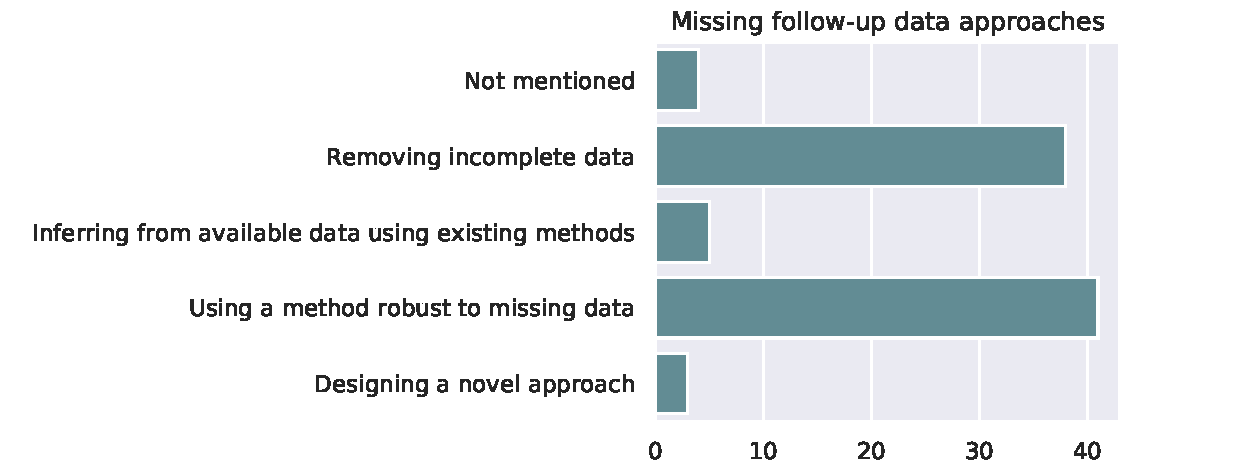
\includegraphics[width=1.0\textwidth]{figures/review/Fig7.pdf}
     \caption{Distribution of papers by their approach to missing longitudinal data.}
     \label{fig:missingfoll}

\end{figure}

Figure \ref{fig:missingfoll} shows the distribution of the works according to the strategy used to deal with missing longitudinal data. We have divided the different approaches into five categories: \\

\begin{itemize}\itemsep7pt

\item \textbf{Not mentioned:} Papers in this category did not report their approach to missing data. It is implied that they used a data cohort without missing entries. However, given the importance of this problem, it is concerning that it was not even mentioned.

\item \textbf{Removing incomplete data:} A solution is selecting only a balanced subset of the available data, removing patients with missing longitudinal acquisitions. This approach has two main problems: it reduces the amount of available data, discards potentially relevant information, and it can introduce biases in the data, especially if they are not missing at random \cite{Lo2012}.

\item \textbf{Inferring from available data using existing methods:} Some works impute missing data from the available cohort, using simple methods such as average value \cite{Zhou2013a} or direct completion from previous time points \cite{Adhikari2019,Huang2016b}, or more complex methods such as sparse regression \cite{Huang2016c} or low-rank matrix completion \cite{Thung2016}. These approaches can be useful to deal with small amounts of random missing data, and they can be used as a preprocessing step, but tend to not scale well and become imprecise with larger amounts \cite{Ibrahim}. 

\item \textbf{Using a method robust to missing data:} In these papers, the method itself accounts for unbalanced data \cite{Liu2015b}. For example, approaches based on mixed effect models, which are robust to missing observations \cite{Donohue14,Schmidt-Richberg2015}, or approaches where each time point is processed separately \cite{guerrero}. Some studies have adapted methods that were not initially flexible to unbalanced datasets. For example, in Adhikari et al.\ \cite{Adhikari2019} they proposed a loss function for their model where only available data were used for its calculation, and Zhu et al.\ \cite{Zhu2016a} defined a temporally structured SVM where different amounts of follow-ups could be used. This approach is more complex than just inferring the data, but can lead to more robust models and to the adaptation of existing methods. 
\item \textbf{Designing a novel approach:} Some works propose novel approaches to data missingness, making it a central point of their work \cite{Dawson2016,Ghazi2019,Goyal2018,Jie2017,Zhu2018}. Those that work with unbalanced data are more broadly applicable: a larger dataset can be used for training/validating the model, and it can be transferred more easily on a clinical setting, where the available data for a given subject may be sparse.

\end{itemize}

Although the majority of the reviewed papers address this important issue, a sizeable proportion ($42.8 \%$) just focus on analyzing curated datasets. This can be useful to showcase new methods and concepts, but not for creating a model that works in a real environment. Adapting existing (cross-sectional) models, such as SVM or DL, to the longitudinal domain \cite{Adhikari2019,Ghazi2019,Jie2017,Zhu2016a} could be a stepping stone to developing novel ML models. \\

\begin{figure}[!htbp]
\centering
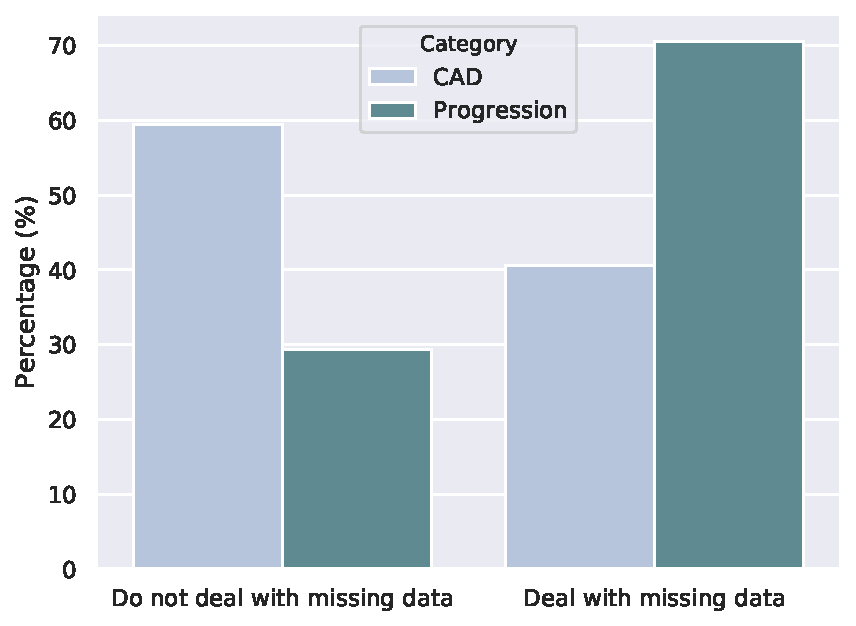
\includegraphics[width=0.65\textwidth]{figures/review/Fig8.pdf}
    \caption[Distribution of the reviewed papers according to whether they deal with longitudinal missing data.]{Distribution of the reviewed papers (categorized by their main aplication) according to whether they deal with longitudinal missing data.}
    \label{fig:missingcat}
\end{figure}

Figure \ref{fig:missingcat} shows the proportion of reviewed papers that deal with missing data (inferring it or using a novel approach or a method robust to it) according to their main objective (either classification for CAD or modelling disease progression). Whereas methods for modelling disease progression can usually deal with unbalanced longitudinal data, classification methods for CAD are more sensitive to missing data.  \\

Multimodal studies need to deal with missing data across modalities, as well as across time. Figure \ref{fig:missingmod} shows the distribution of works according to the strategy used to handle missing data in multimodal studies. Some of them also appear in Figure \ref{fig:missingfoll}, as they deal with both types of data imbalance \cite{Adhikari2019,Goyal2018,Iturria-Medina2016,Jedynak2012}. Almost half of the studies chose not to use subjects with incomplete data, whereas the other half used more flexible methods. As before, progression models based on mixed effect models and other statistical modelling approaches are robust \cite{Iturria-Medina2016,Jedynak2012,Schmidt-Richberg2015,Villemagne2013}, whereas supervised learning approaches for classification are more rigid \cite{Vounou2012,Young2014,Zhang2012a}. \\

\begin{figure}[!htbp]
     \centering
     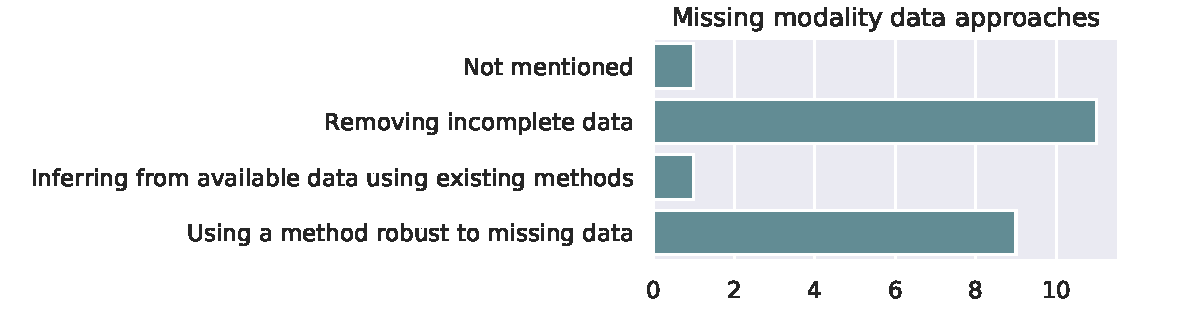
\includegraphics[width=1.0\textwidth]{figures/review/Fig9.pdf}
     \caption[Distribution of papers by their approach to missing multimodal data.]{Distribution of papers by their approach to missing multimodal data. Only multimodal works were considered.}
     \label{fig:missingmod}
\end{figure}

A considerable number of articles \cite{Chen2011b,Chen2012,Eshaghi2017,Hyun2016,Li2013,Li2017b,Zhang2014,Ziegler2015b} used simulated data to test their algorithm for other types of data. This approach allows researchers to create specific scenarios to evaluate the robustness of their algorithms; for example, with a large amount of missing data, with only short-term longitudinal data, or with additional imaging modalities. \\

\section{Reproducibility and interpretability}
\label{sec:bias}

For all studies, results and methods should be reproducible to 1) ensure that the results are legitimate, 2) be able to directly apply the method to other datasets, and 3) facilitate dissemination and open science. Moreover, if the model is to improve diagnosis or better understand the progression of the disease, it needs to be open and interpretable, that is, able to identify the factors that are responsible for triggering a concrete response. \\

Some measures to  ensure the reproducibility of the published results and methods are:

\begin{itemize}\itemsep7pt
\item Using standardized datasets: some studies \cite{cuingnet,Moradi2015,Sanroma2017,Wyman2013} propose or use a concrete set of patients so that anyone can work with the same data. However, such standardized datasets have yet to be widely adopted, as the majority of the reviewed works either use private datasets or do not precise which data are used from public datasets.

\item Using standardized data management for neuroimage storing and sharing, such as BIDS\footnote{\url{https://bids.neuroimaging.io/}}. 

\item Using methods such as cross-validation to minimize overfitting \cite{Yang2018}.

\item Reproducing methods on a completely different cohort of patients to test the robustness of the results \cite{Casanova2018}.

\item Making the code used to generate the code publicly available.
\end{itemize}

We studied the reproducibility of the reviewed works by checking if the code and the data to generate the model and the reported results are available. We considered that data were reported if they were directly available, or they could be obtained without ambiguity from a public dataset. As shown in Figure \ref{fig:reproduc}, although some papers make their data available, very few ($15.3 \%$) include the code. Most papers report neither data nor code.  \\

\begin{figure}[!htbp]
\centering
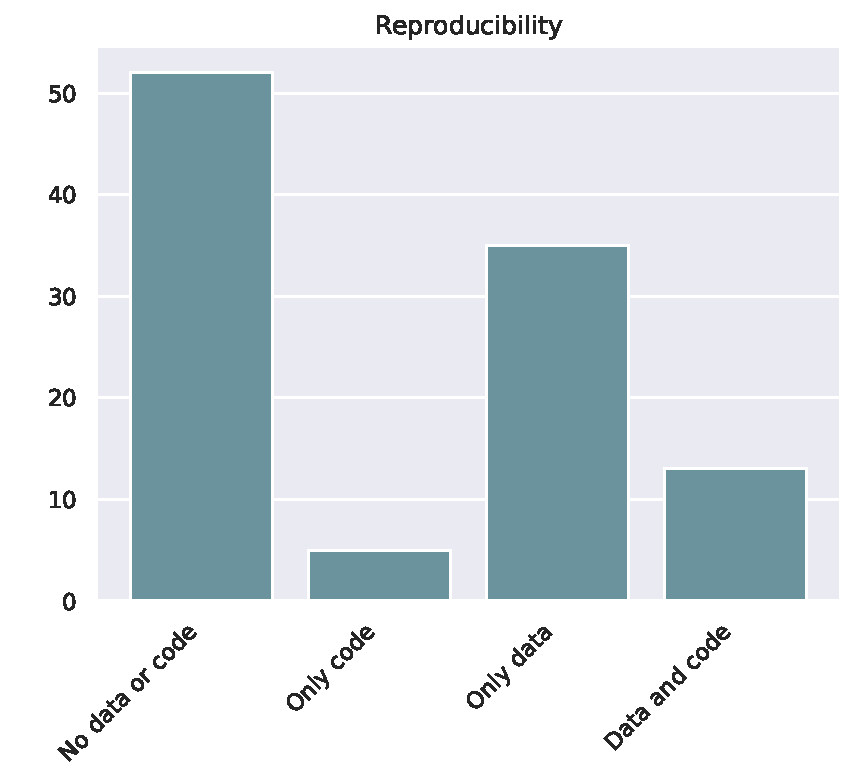
\includegraphics[width=0.65\textwidth]{figures/review/Fig10.pdf}
    \caption[Distribution of the reviewed papers by their reproducibility.]{Distribution of the reviewed papers by their reproducibility. Vertical axis indicates amount of papers.}
    \label{fig:reproduc}
\end{figure}

Regarding interpretability, some ML methods, such as DL, have been criticized for being a black box \cite{Ching2018}, not providing the underlying reasoning of the model. Interestingly, many of the reviewed works chose ML methods allowing some level of interpretability, which is crucial for clinical use. Most of the disease progression models are interpretable since their underpinning aim is to obtain a clinically interpretable representation of the disease pathophysiology. Other examples are methods based on MKL \cite{Chen2015,Gonen2011,Zhang2012a}, where biomarkers are assigned a weight according to their importance to the learned task, or manifold learning methods \cite{Guerrero2015,guerrero,Wolz2010}, where patients can be embedded in a low-dimensional space to directly visualize the relationships between them.

\section{Discussion}
\label{sec:conclusion}

We have surveyed papers that use ML algorithms for longitudinal data analysis. Most of the works focus on neuroimaging, mainly MRI. A significant percentage of the works (approximately $26\%$) use multimodal data. Although the reviewed papers target various tasks, we can divide them into two groups: disease progression modelling and CAD. Methods for disease progression modelling can usually deal with unbalanced longitudinal data, whereas CAD methods are more sensitive to missing data. \\

For some specific problems, such as classification between converting and non-converting MCI, longitudinal data showed a strong performance \cite{Liu2013,Sun2017}, compared to standard cross-sectional methods \cite{cuingnet}. Better detection of MCI converters could lead to improved early detection of the disease, through the development of novel methods that help prevention policies, and longitudinal epidemiological studies that focus on early stages and healthy subjects. Since AD affects different biological processes, multimodal studies provide a more comprehensive view of the disease. Studies using more than one modality are gaining importance \cite{Chen2015,Chi2017,Hinrichs2011,Minhas2016,Zhang2012a}, and results in specific problems, such as classification in CAD systems, have shown a slight improvement compared to single modality studies. There is enough evidence from existing multimodal studies \cite{Iturria-Medina2016,Jedynak2012,Oxtoby2018} that integrating those different sources can boost performance. \\

Based on our analysis, we argue that methods should aim for robustness to missing and unbalanced data, especially for CAD applications. Among the different approaches to tackle this problem, a promising one is using simulated data \cite{Chen2011b,Chen2012,Eshaghi2017,Hyun2016,Li2017b,Li2013,Zhang2014,Ziegler2015b}. This allows validating a model in different settings and testing its robustness for different rates of unbalanced/missing data, or setting baseline before using real data. \\

To improve understanding of the disease and make the methods rigorous and applicable to a clinical setting, more effort towards reproducibility and interpretability of the methods and results is needed. A more widespread use of validation tools and cohorts would be desirable. Many papers do not use standardized datasets, nor share their data, so their results are hard to compare with other works. Moreover, some of the papers rely on "hard-to-interpret" ML techniques \cite{Givon2017,Zhang2017}. \\

Despite large advances in longitudinal data analysis, more research is necessary on methods that better process and interpret the large influx of relevant information that a longitudinal characterization of the disease can offer. Prior knowledge or assumptions of the disease should be incorporated to naturally accommodate longitudinal data \cite{Fonteijn2012,Gavidia-Bovadilla2017,Zhu2016a}. In this context, the ATN biomarker framework \cite{Jack2018}, which provides a biologically based definition of AD opens up a new path to more accurately characterize the disease. \\

Regarding CAD applications, DL approaches have achieved great success in medical imaging \cite{Litjens2017}, in brain disease diagnosis \cite{Talo2019,Talo2019b}, and more specifically in AD \cite{Liu2014,Jo2019}, using cross-sectional imaging data. However, our findings show that their application for longitudinal analysis is still low (only $6\%$ of the reviewed articles used DL based techniques). Incorporating longitudinal neuroimaging data to DL classification systems is challenging due to the high dimensionality that a temporal dimension adds. Moreover, it is not straightforward to solve the problem of missing data and variable number of follow-ups in a multi-layer architecture, as several works addressing this problem show \cite{Givon2017,Ghazi2019}. More work should be done to incorporate such techniques to the study of longitudinal, high dimensional neuroimaging data, where they hold promise for better understanding and treatment of the disease. Given the aforementioned success and great performance of DL for cross-sectional studies, we encourage and expect advancements in DL based systems using longitudinal data in the near future.\\

Almost all reviewed papers use supervised methods. Unsupervised (or semi-supervised) learning could be useful in dealing with longitudinal data, where data are usually unbalanced or not labelled in some of the modalities. Clustering or other unsupervised techniques, for example, could be used to study the relationships between different trajectories of patients, without relying on labels or large amounts of data.  \\

More research to overcome the described problems and challenges is key to broaden our understanding of the progression of AD and other neurodegenerative diseases. These methodological advances would open the door to developing applications that can be useful in clinical and epidemiological settings.

\section*{Acknowledgements}
This research was partially funded by the “Fundació La Marató de TV3” (nº20154031). This work was also funded by the Spanish Ministry of Economy and Competitiveness under the María de Maeztu Units of Excellence Programme [MDM-2015-0502]. The authors declare that they have no known competing financial interests or personal relationships that could have appeared to influence the work reported in this paper.\\